\chapter{Umsetzung}
\section {Idee und Konzeption}
Meine Idee ist ein Videospiel zu entwickeln, das eine geschichtliche und kulturelle Relevanz zur deutschen Geschichte hat. Ein weiteres Kriterium an meinem Videospiel ist es, ein Szenario zu wählen, das sich vor dem Zweiten Weltkrieg befindet. Mit dieser Idee habe ich folgenden Prompt für ChatGPT formuliert und anschließend dien in Abbildung \ref{ersten-5-themen}Ausgabe bekommen.
\begin{figure}[h]
   		 \centering
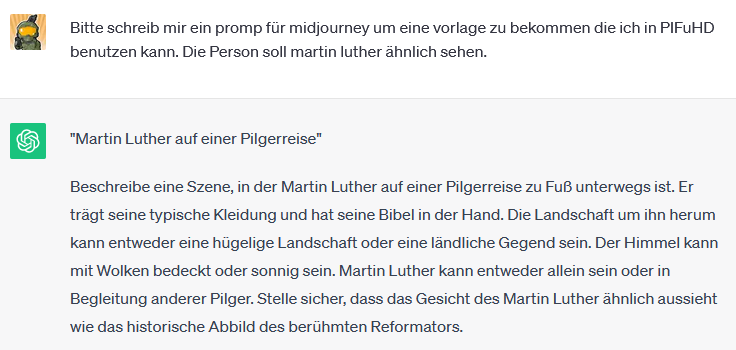
\includegraphics[width=14cm]{BilderFuerBA/01.png}
   		 \caption{Ersten fünf Themen}
   		 \label{ersten-5-themen}
\end{figure}
\\
Nachdem ich mit den ersten 5 Ideen von ChatGPT nicht zufrieden habe ich mir weitere 5 Themen ausgeben lassen die in Abbildung \ref{zweiten-5-themen}.
\begin{figure}[h]
   		 \centering
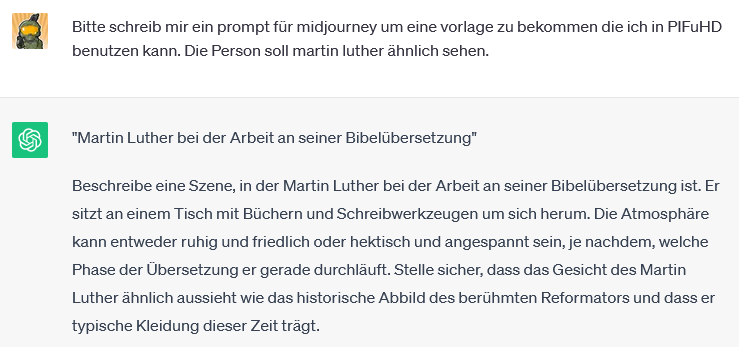
\includegraphics[width=14cm]{BilderFuerBA/02.png}
   		 \caption{ChatGPT: Zweiten fünf Themen}
   		 \label{zweiten-5-themen}
\end{figure}
Man kann an diesem Beispiel sehen, dass ChatGPT mir 10 Ideen präsentiert, die ich in meinem Videospiel verarbeiten kann.
\\
Als Ein-Mann-Videospielentwickler entschied ich mich für die Reformation mit Martin Luther als Hauptfigur.
\\
Innerhalb dieser Bachelorthesis ist es mir aus Zeitgründen nicht möglich ein komplettes Videospiel zu entwickeln, was das Leben von Martin Luther widerspiegelt. Durch meine Recherche über Martin Luther und sein Leben fand ich den Moment bedeutend wo Martin Luther seine 96 Thesen an das Kirchtor nagelt.
\\
In meinem Prototyp werde ich dieses Ereignis als Thematischen Mittelpunkt wählen.
\\
Meine Spielidee für meinen Prototyp ist nun, dass Martin Luther durch ein Dorf läuft, verschiedene NPCs trifft und mit ihnen in einen Dialog tritt. Martin Luther trifft verschiedene Personen mit verschiedenen Problemen und Ansichten. Er redet mit ihnen und lässt sich von ihnen inspirieren. Durch diese Inspiration entwickelte Martin Luther später im Spiel, seine 96 Thesen.
\\
Kern des Prototyps ist die Entwicklung einer Spielwert, die aus einem Dorf mit verschiedenen Häusern und NPCs besteht.
\\
Die Entwicklung des Prototyps unterteilt sich in verschiedene Meilensteine:
-Hauptfigur
\\
-Landschaft
\\
-Gebäude
\\
-Nebenfiguren
\\
-Dialogsystem
\\
-Sprachausgabe
\\
Jeder dieser Meilensteine besitzt in dieser Theses sein eigenes Kapitel, in dem die Entwicklung nahegebracht wird.

%\\\\\\\\\\\\\\\\\\\\\\\\\\\\\\\\\\\\\\\\\\\\\\\\\\\\ HUPTFIGUR\\\\\\\\\\\\\\\\\\\\\\\
%\\\\\\\\\\\\\\\\\\\\\\\\\\\\\\\\\\\\\\\\\\\\\\\\\\\\ HUPTFIGUR\\\\\\\\\\\\\\\\\\\\\\\
%\\\\\\\\\\\\\\\\\\\\\\\\\\\\\\\\\\\\\\\\\\\\\\\\\\\\ HUPTFIGUR\\\\\\\\\\\\\\\\\\\\\\\
\section {Meilenstein: Hauptfigur}
\begin{figure}
	 \centering
	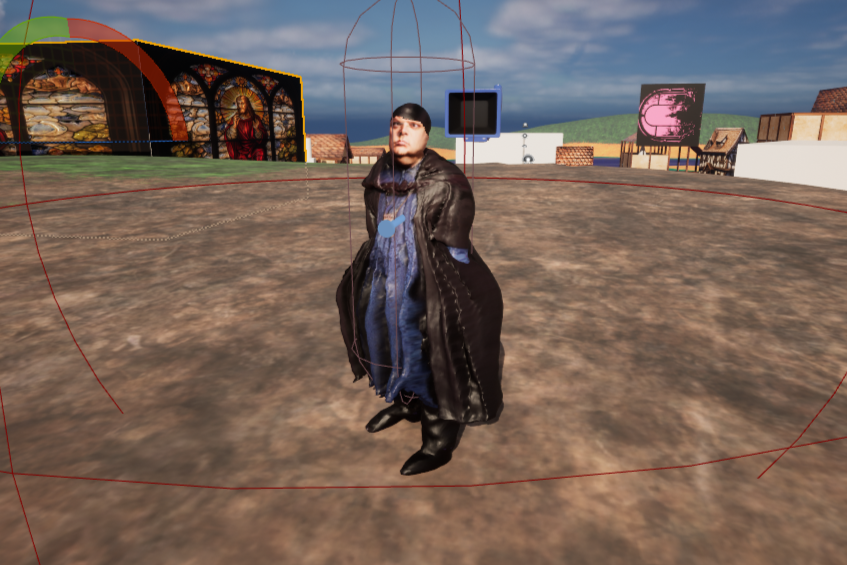
\includegraphics[width=14cm]{BilderFuerBA/MartinLutherImSpiel.png}
	\caption{UE5: Martin Luther im Spiel}
	\label{MartinLutherImSpiel}
\end{figure}

\begin{figure}
	\centering
	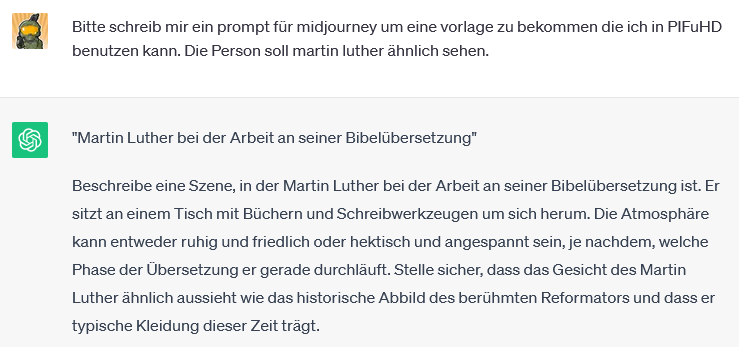
\includegraphics[width=14cm]{BilderFuerBA/02.png}
	\caption{ChatGPT: Erster Versuch zur erstellung eines Promt für Midjourney}
	\label{ChatGPT_erster_Versuch_Midjourney_Promt}
\end{figure}

\begin{figure}
	\centering
	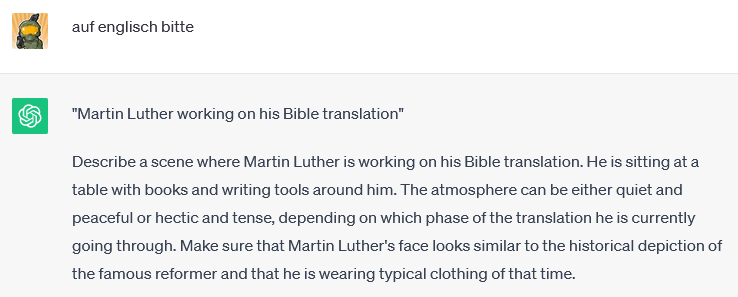
\includegraphics[width=14cm]{BilderFuerBA/03.png}
	\caption{ChatGPT: Übersetzung des Prompts}
	\label{ChatGPT_übersetzen}
\end{figure}

\begin{figure}
	\centering
	\begin{minipage}[t]{0.45\linewidth}
		\centering
		\includegraphics[width=6.405cm]{BilderFuerBA/Busfahrer.png}
		\caption{Midjourney Prompt: Bussfahrer}
		\label{Bussfahrer}
	\end{minipage}
	\hfill
	\begin{minipage}[t]{0.45\linewidth}
		\centering
		\includegraphics[width=6.405cm]{BilderFuerBA/bus_driver.png}
		\caption{Midjourney Prompt: bus driver}
		\label{bus_driver}
	\end{minipage}
\end{figure}



\begin{figure}
    \centering
    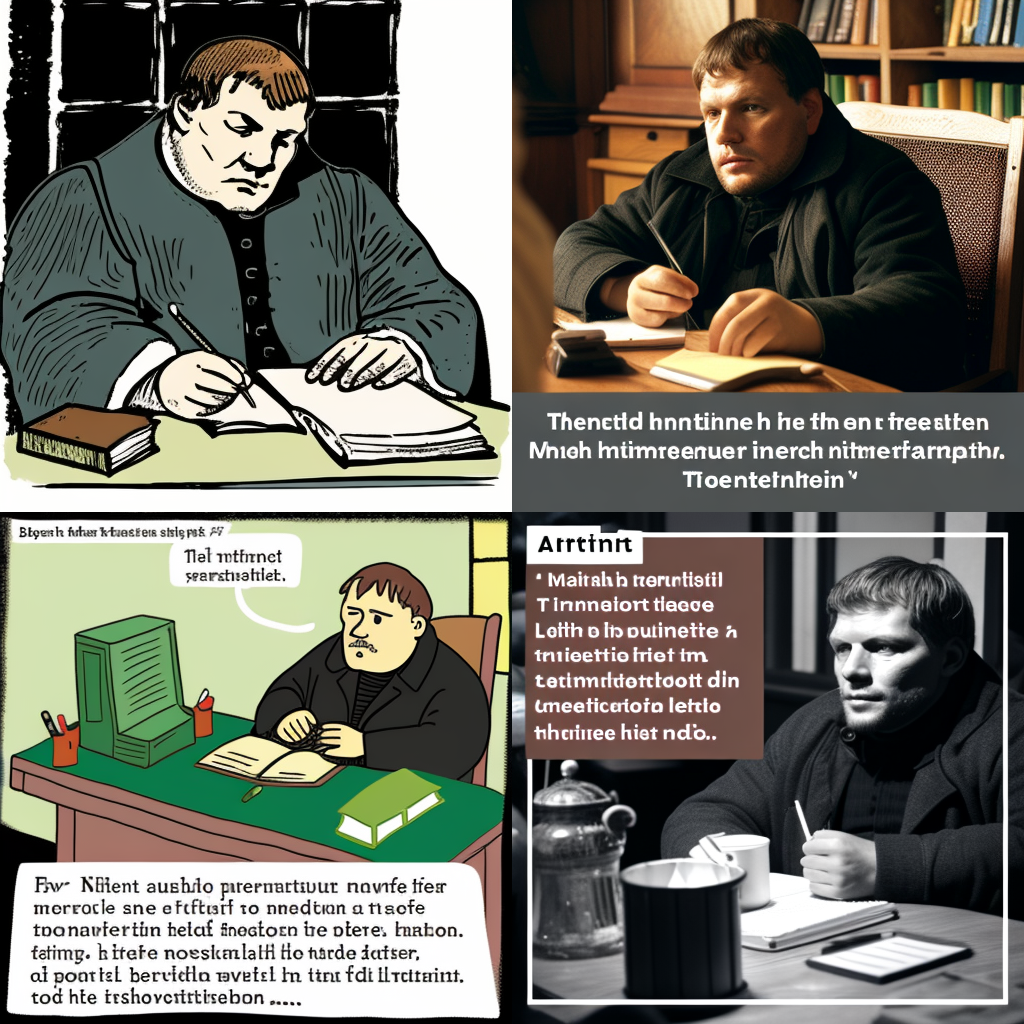
\includegraphics[width=8.022cm]{BilderFuerBA/MLaufEnglisch.png}
    \caption{Midjourney: Erster Prompt von ChatCPT}
    \label{Midjourney_erster_Prompt}
\end{figure}

\begin{figure}
    \centering
    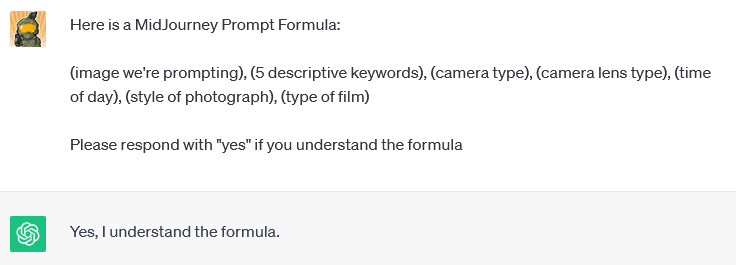
\includegraphics[width=14cm]{BilderFuerBA/04.png}
    \caption{ChatGPT: Aufforderung verwendung einer Midjourney-Formel}
    \label{chatgpt-ptompt-Midjourney-04}
\end{figure}
\begin{figure}
    \centering
    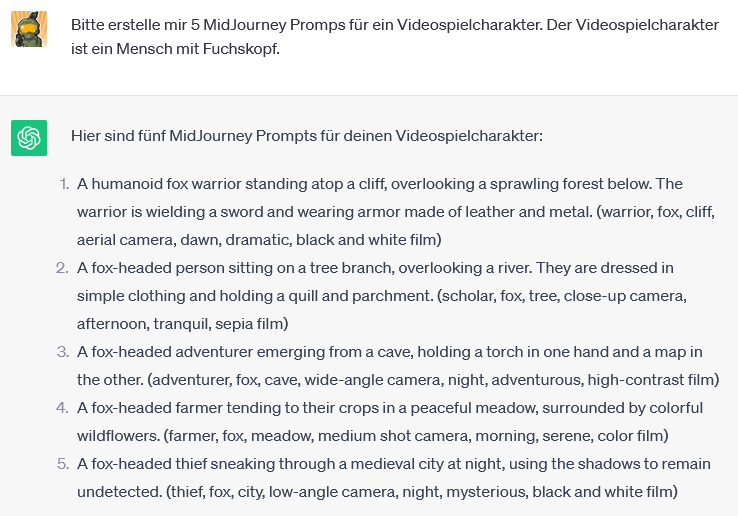
\includegraphics[width=14cm]{BilderFuerBA/05.png}
    \caption{ChatGPT: Erstellung Prompts mit Verwendung der Midjourney-Formel}
    \label{chatgpt_mj-formel_mit_Klammern}
\end{figure}

\begin{figure}
	\centering
	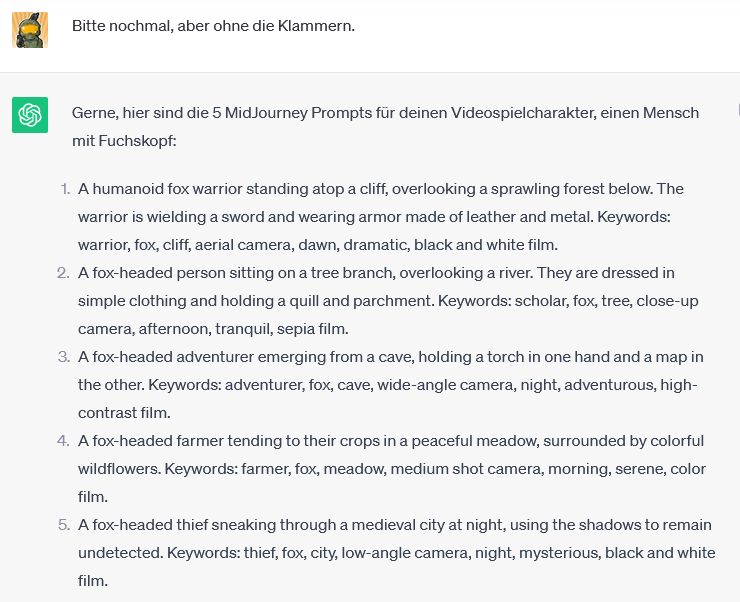
\includegraphics[scale=0.7]{BilderFuerBA/06.png}
	\caption{ChatGPT: ChatGPT erstellt Promt für Midjourney in Englisch und ohne Klammern}
	\label{chatgpt_mj-formel_ohne_Klammern}
\end{figure}

\begin{figure}
	\centering
	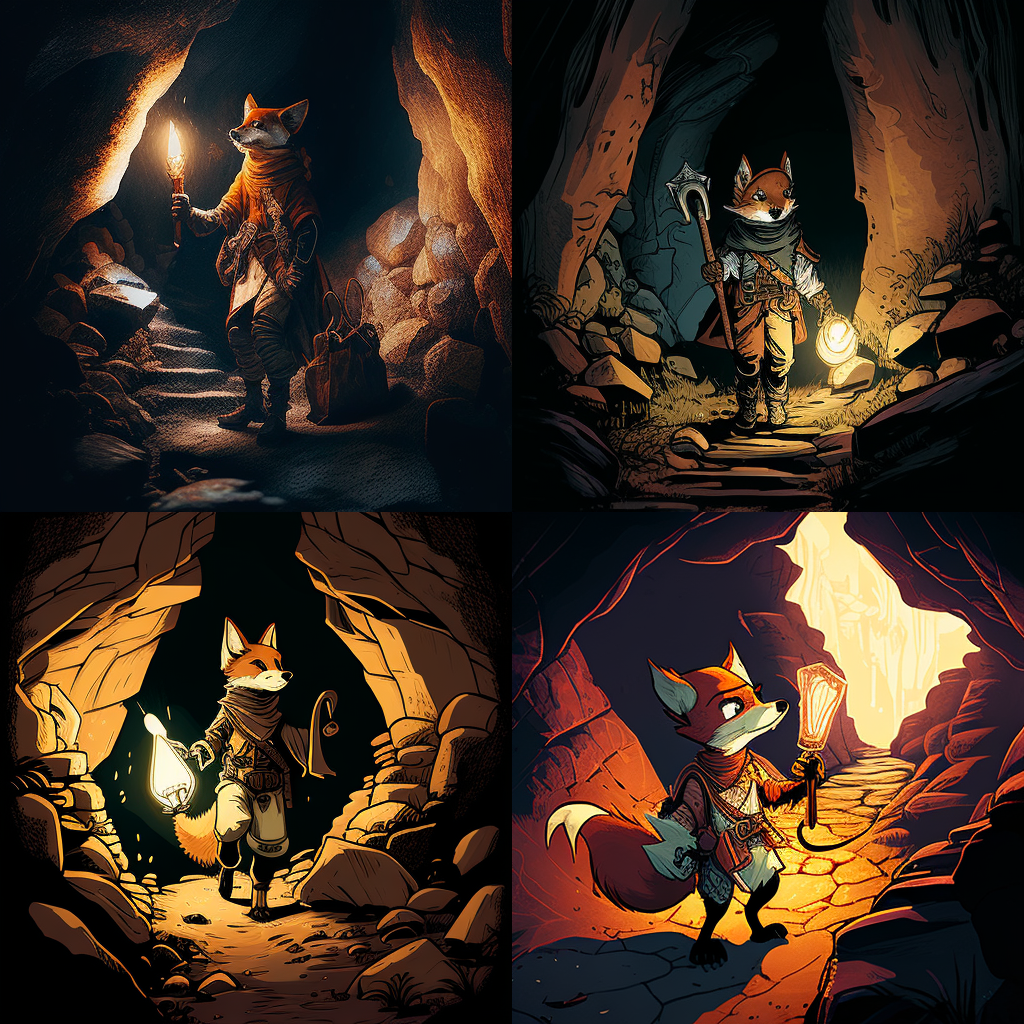
\includegraphics[width=8.022cm]{BilderFuerBA/fuchsKopfAbenteuerer.png}
	\caption{Midjourney: Promt eines Abenteurers mit einem Fuchskopf}
	\label{MidjourneyFuchsKopfAbenteuerer}
\end{figure}

\begin{figure}
	\centering
	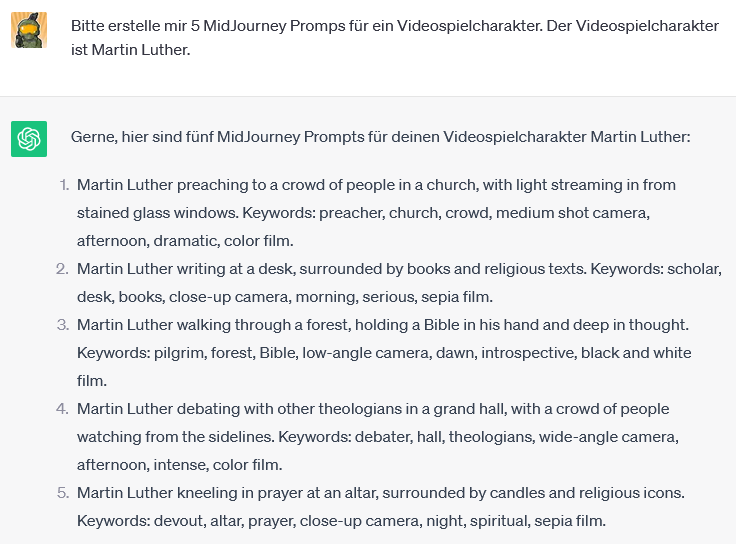
\includegraphics[scale=0.7]{BilderFuerBA/07.png}
	\caption{ChatGPT: Midjourney Prompt für Martin Luther als Spielfigur}
	\label{chatgptMartinLutherMJformelErstenFünf}
\end{figure}


\begin{figure}
	\centering
	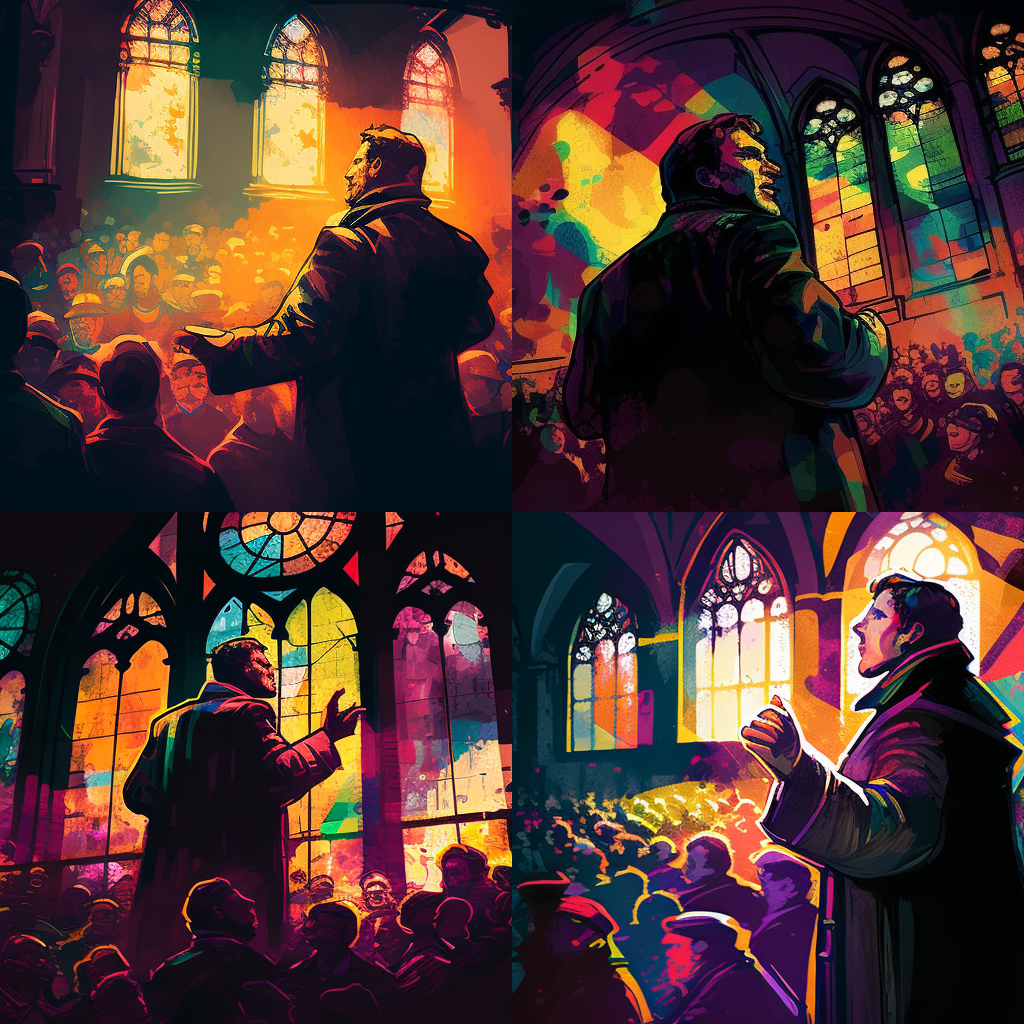
\includegraphics[width=8.022cm]{BilderFuerBA/MidJourneyMLMitFormel.png}
	\caption{Midjourney: Martin Luther Promt mit Midjourney-Formel}
	\label{MidJourneyMLMitFormel}
\end{figure}

\begin{figure}
	\centering
	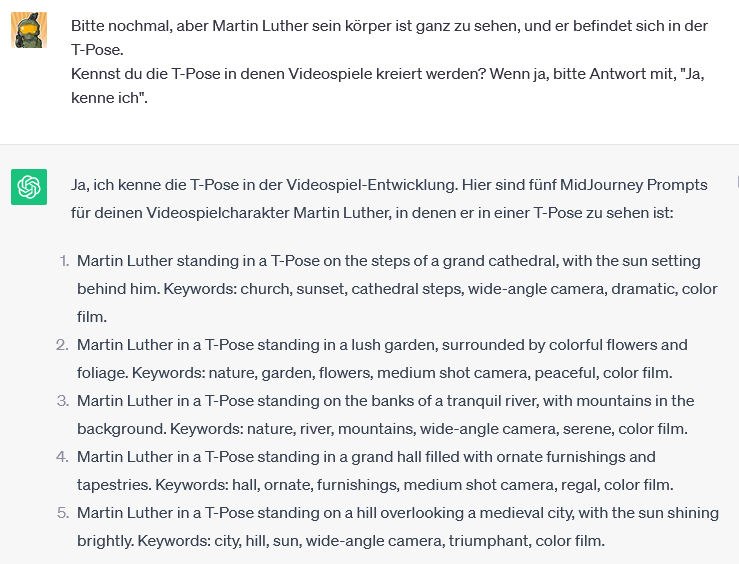
\includegraphics[scale=0.7]{BilderFuerBA/09.png}
	\caption{ChatGPT: Midjourney Prompt für Martin Luther in T-Pose}
	\label{chatgptMartinLutherMJinTPose}
\end{figure}

\begin{figure}
	\centering
	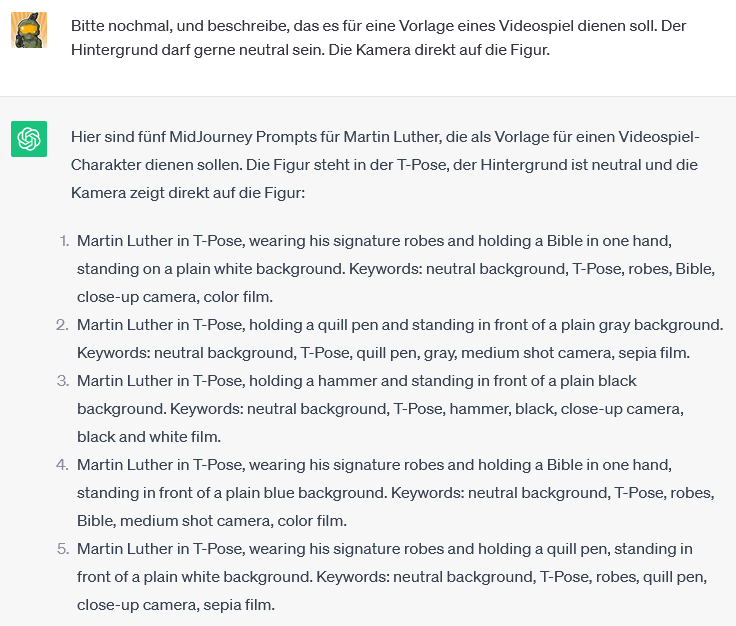
\includegraphics[scale=0.7]{BilderFuerBA/10.png}
	\caption{ChatGPT: Midjourney Prompt für Martin Luther in T-Pose}
	\label{chatgptMartinLutherMJmitNeutralenHintergrund}
\end{figure}

\begin{figure}
	\centering
	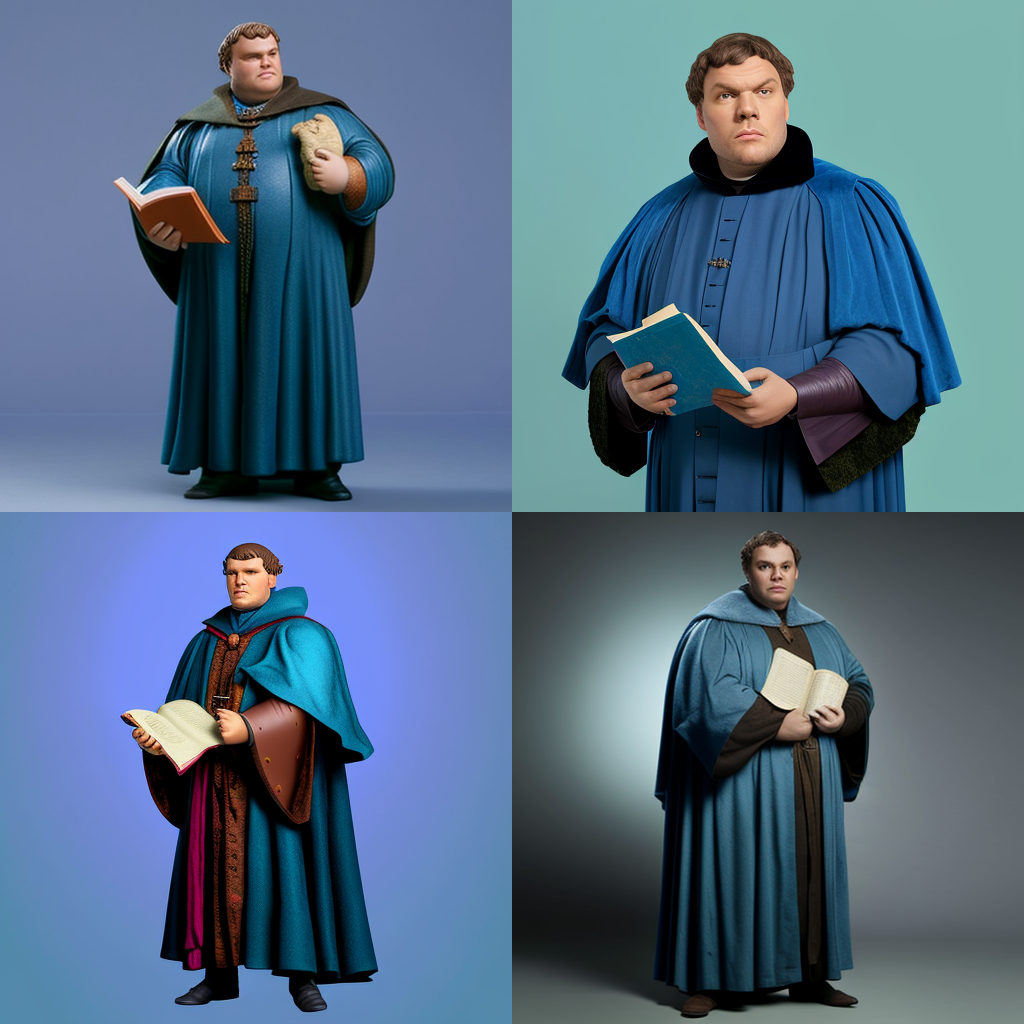
\includegraphics[width=8.022cm]{BilderFuerBA/MartinLutherInTPoseFirst.png}
	\caption{Midjourney: Martin Luther Promt versuch in T-Pose, neutralen Hintergrund und direkte Kamera}
	\label{MartinLutherInTPoseNeutralerHintergrundDirekteKamera}
\end{figure}

\begin{figure}
	\centering
	\includegraphics[width=8.022cm]{BilderFuerBA/ErsteAusgabeVomFinalenPrompt.png}
	\caption{Midjourney: Erste Ausgabe vom finalen Prompt}
	\label{ErsteAusgabeVomFinalenPrompt}
\end{figure}

\begin{figure}
	\centering
	\includegraphics[width=8.022cm]{BilderFuerBA/ZweiteAusgabeVomFinalenPrompt.png}
	\caption{Midjourney: Vier weitere Variation von Version Zwei}
	\label{ZweiteAusgabeVomFinalenPrompt}
\end{figure}

\begin{figure}
	\centering
	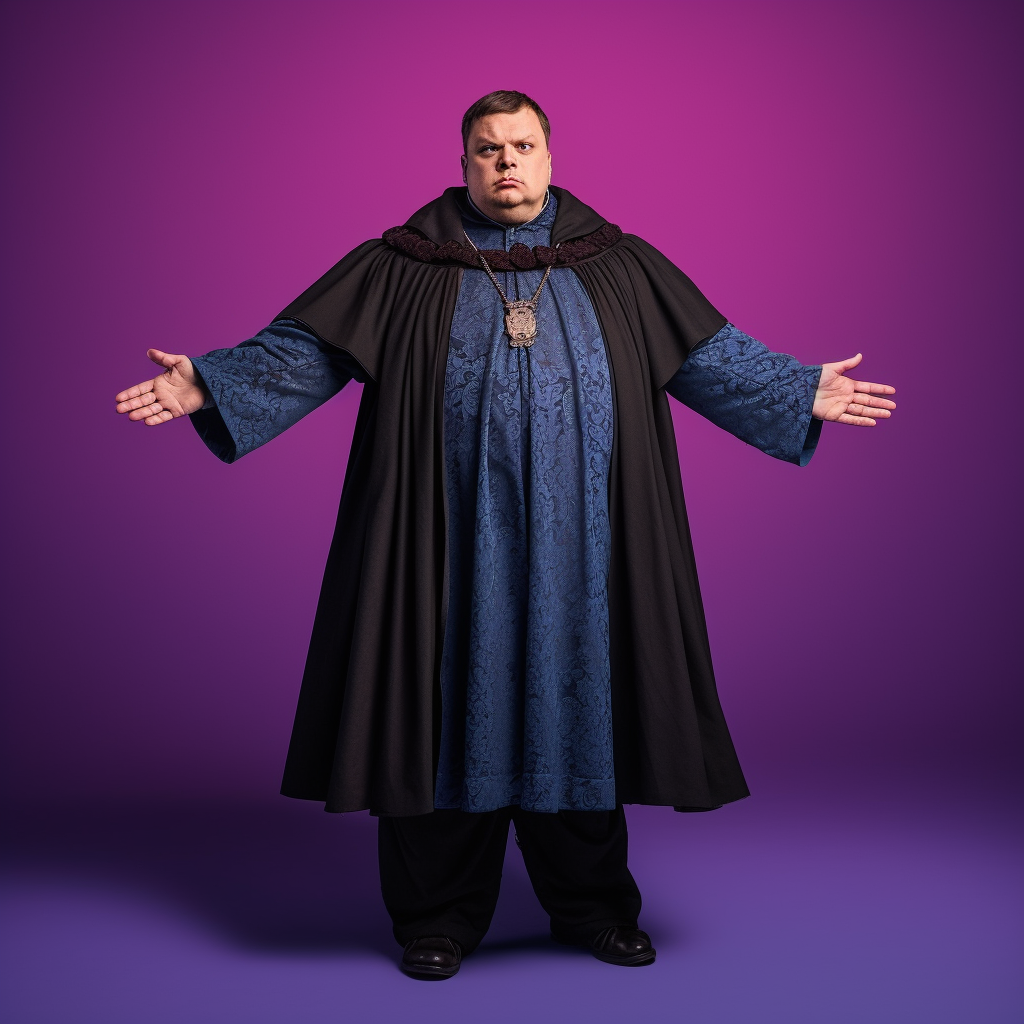
\includegraphics[width=8.022cm]{BilderFuerBA/DritteAusgabeVomFinalenPrompt.png}
	\caption{Midjourney: Hochskaliertes Endresultat von Version Vier}
	\label{DritteAusgabeVomFinalenPrompt}
\end{figure}

Auf Abbildung \ref{MartinLutherImSpiel} ist die Huptspielfigur des Prototypes zu Sehen. Die Hauptfigur ist Martin Luther nachempfunden. Die Hauptspielfigur ist vom Spieler Steuerbar und wurde mit Hilfe den KI-Systemen ChatGPT, Midjourney und PIFuHD erstellt. Wie die soben genannten KI-Systeme verwendet wurden, werde ich in den folgenden Absätzen ausfühlich erklären
\\
Ich beginne die Entwicklung der Hauptfigur in dem ich ChatGPT um eine Beschreibung meiner Hauptfigur auffordere. Ich gebe ebenfalls an, dass ich die Ausgabe von ChatGPT als Prompt für Midjourney verwenden möchte. Zusätzlich fordere ich ChatGPT auf, dass das Ergebnis von Midjourney für PIFuHD kompatibel sein soll.
\\
Mit der in Abbildung \ref{ChatGPT_erster_Versuch_Midjourney_Promt} zusehenden Aufforderung, habe ich eine deutsche Ausgabe bekommen. Durch eine weitere kurze Aufforderung wie in Abbildung \ref{ChatGPT_übersetzen} wurde die Ausgabe von ChatGPT übersetzt.
\\
Midjourney liefert in Englisch in Gegensatz im Vergleich zu Deutsch oft unterschiedliche Ergebnisse. Beobachten kann das zum Beispiel in Abbildung \ref{Bussfahrer} Bussfahrer auf deutsch, und in Abbildung \ref{bus_driver} buss driver auf englisch.
\\
Anhang in Abbildung \ref{Bussfahrer} und Abbildung \ref{bus_driver} kann man gut beobachten, dass die verwendeten Sprache ein Unterschied macht. Im Englischen wird eher eine Person dargestellt, die ein Lenkrad in der Hand hält, wo der Prompt auf deutsch eher ein Passagier dargestellt wird oder ein Bus in einer Landschaft.
\\
%https://philipp-stelzel.com/de/midjourney-deutsch-sprachen/ Abrufdatum 25.09.2023
Midjourney versteht nicht unsere Sprache, sondert die Genauigkeit entsteht aus der Menge der Daten womit das KI-System Trainiert ist. Das Wort Bussfahrer kommt womöglich mit nicht so oft in den Trainigsdaten vor wie buss driver aus dem Englischen.
\\
Mit dieser Erkenntnis, entscheide ich mich meine Promts auf Englisch für Midjourney zu verfassen bzw von ChatGPT verfassen lassen.
\\
Nach der Übersetzung von ChatGPT, übergebe ich den von ChatGPT generierten Promt Midjourney. Das Ergebnis is in Abbildung \ref{Midjourney_erster_Prompt} zu betrachen.
\\
In Abbildung \ref{Midjourney_erster_Prompt} ist zu sehen, das Midjourney immer Vier bilder als Vorschau ausgibt. Midjourney bietet über sein User-Interface drei Möglichkeiten um mit dem Ergebnis weiter zu Arbeiten.
\begin{itemize}
	\item 1 Vier weitere Versionen auf grundlage von Version 1 bis 4
	\item 2 Eine Hochskallierte Version von 1 bis 4
	\item 3 Vier neue weitere Versionen
\end{itemize}
Oben links befindet sich Version 1, oben rechts Version 2, unten links Version 3 und unten rechts Verion 4.
\\
Der Prompt von ChatGPT aus Abbildung \ref{ChatGPT_übersetzen} beinhaltet sehr viele Schlüsselwörter die in Textform verfasst sind. Ich beschreibe den Promt von ChatGPT sehr Athomsphärisch, wie als würde man eine Textstelle aus einem Roman lesen, anstelle einer Aufforderung gegenüber eines KI-System.
\\
Ich vermutet, dass ChatGPT nicht genügend darauf trainiert ist, wie Midjourney-Prompts auszusehen haben.
\\
Eine Recherche auf YouTube hat gezeigt, dass das Verwenden von Midjourney-Formeln ein aufgeräumtes Ergebnis hervorbringen kann. Eine Kurze Auforderung wie in Abbildung \ref{chatgpt_formel_mj_first_5} kann bessere Ergebnisse bei Midjourney gewähren.
\\
Im ersten Test werden die Prompts mit Klammern \ref{chatgpt_mj-formel_mit_Klammern} ausgegeben. Diese sind mit einer einfachen Aufforderung wie in \ref{chatgpt_mj-formel_ohne_Klammern} möglich zu entfernen.
\\
Ich habe die Ausgabe mit dem Fuchskopf Midjourney übergeben und das ergebnis ist in Abbildung \ref{MidjourneyFuchsKopfAbenteuerer} zu sehen.
\\
Da mein Hauptcharakter kein Abenteurer mit Fuchskopf ist, sonder Martin Luther nachempfunden sein soll, habe ich ChatGPT dazu Aufgefordert mir 5 Promts für Midjourney zu erstellen um Bilder von Martin Luther generieren zu lassen. Die Ergebnisse von ChatGPT ist in Abbildung \ref{chatgptMartinLutherMJformelErstenFünf} zu sehen. Die dazu entstandenen Bilder von Midjourney sind in Abbildung \ref{MidJourneyMLMitFormel} zu sehen.
\\
Der Vorteil dieser Methode ist, das man nun einzelne Parameter in der Midjourney-Formel belieben verändern kann um ein Gewünschtes Ergebnis zu erlangen. Das Ziel ist es ein "Foto" von Martin Luther zu bekommen um es später für PIFuHD zu verwenden. Das Ergebnis von Abbildung \ref{MidJourneyMLMitFormel} ist noch nicht zu verwenden, da zu viele Fabenfrohe Deteils zu sehen sind. PIFuHD weist darauf hin das Bilder am besten funktionieren wenn die zu verwendeten Bilder:
\begin{itemize}
	\item eine Mindestauflösung von 512 x 512 Pixel haben.
	\item nur eine Person zeigt und direkt in die Kamera schaut.
	\item gut beleuchtet ist.
	\item einen einfachen Hintergrund besitzen.
\end{itemize}

Um diese Punkte zu beachten habe ich folgende Parameter von ChatGPT überarbeiten lassen. Als erstes soll der Charakter in der T-Poste stellung sein Abbildung \ref{chatgptMartinLutherMJinTPose} anschließend mit einem Neutralen Hintergrund und einer direkten Kamere auf die Figur. Das Ergebnis ist in Abbildung \ref{MartinLutherInTPoseNeutralerHintergrundDirekteKamera} zu sehen.
\\
An dieser Stelle habe ich nicht mehr mit ChatGPT für die Hauptfigur gearbeitet. Ab hier habe ich sehr viel ausprobiert um eine Fotoähnliche abbildung von Martin Luther zu bekommen. Der Finale Prompt der am ende das Bild von Martin Luther generiert hat war:
\\
\rmfamily
\begin{large}
	the famous martin luther from germany, robe from the Renaissance, T-Pose for gamedesign, standing in front of a plain blue background. neutral magenta background, T-Pose, whole body, face looking in the camera, color film
\end{large}
\sffamily
\\
Midjourney
\\
Mit diesem Prompt habe ich es geschafft mit Version 2 in Abbildung \ref{ErsteAusgabeVomFinalenPrompt} ein Ergebnis zu generieren was meine Anforderung als Game Designer entprechen. Ich habe ein, gerade in die Kamera schauende Mann der Martin Luther ähnlich sieht. Der Mann steht in einer T-Pose. Der Hintergrund ist farbarm / neutral und wir sehen den kompletten Körper.
\\
Durch die betätigung des Buttons V2 bekomme ich 4 weiter Versionen auf grundlage von Version 2 aus der Abbildung \ref{ErsteAusgabeVomFinalenPrompt}.
\\
Abbildung \ref{ZweiteAusgabeVomFinalenPrompt} zeigt vier weitere Versionen von Version 2 der Ausgabe \ref{ErsteAusgabeVomFinalenPrompt}. Die Unterschiede sind viel geringer und unterscheiden sich in diesem Beispiel am größten an der Frisur, den Oberteil der Robe und der Kette. Den rest empfinde ich sehr ähnlich.
\\
Besonder die Kette ist ein Deteil was mich als Game Designer am meisten angesprochen hat, was mich am Ende dazu entschieden hat, Version Vier über den Button U4 hochzuskaliern.
\\
Die hochskalierte Version von Abbildung \ref{ZweiteAusgabeVomFinalenPrompt} ist in Abbildung \ref{DritteAusgabeVomFinalenPrompt} zu betrachten.
\\
Wir sehen einen Mann in einer Kirchlich anmutenen Robe. Sein Haar ist braun, seine Haut hell. Der Mann trägt beide Arme vom Körper so das die Handinnenfläche zur Kamera zeigen.
\\
Dieses Bild verwende ich um ein 3D-Modell von Martin Luther zu verwenden.
\subsection{Erzeugen eines 3D-Modells mit Hilfe von PIFuHD}
\begin{figure}
	\centering
	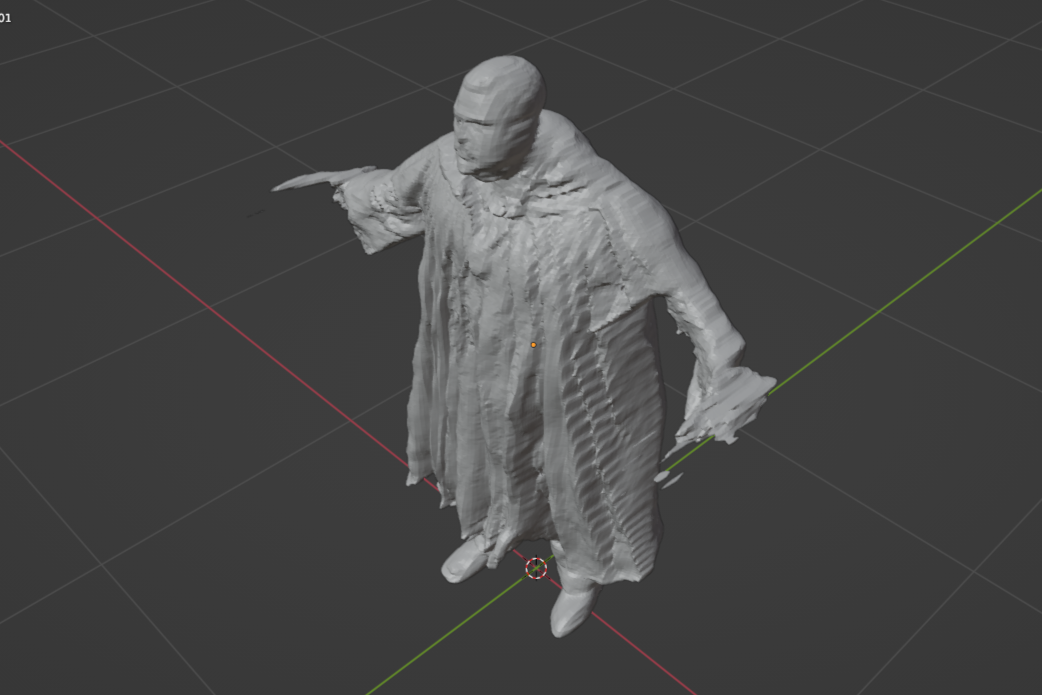
\includegraphics[width=14cm]{BilderFuerBA/BlenderMLVonPIFuHD105k.png}
	\caption{Blender: 3D-Modell von Martin Luther von PIFuHD}
	\label{BlenderMLVonPIFuHD105k}
\end{figure}
\begin{figure}
	\centering
	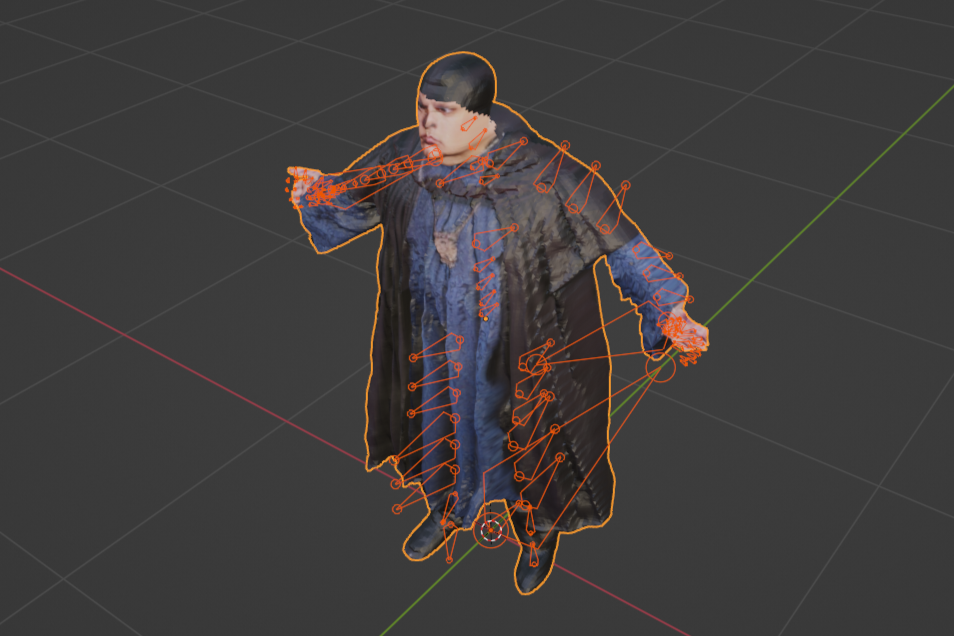
\includegraphics[width=14cm]{BilderFuerBA/BlenderMLGeriggtUndTexturiert95k.png}
	\caption{Blender: Martin Luther Texturiert, geriggt, Nachgebessert und gemergeten Verticies}
	\label{BlenderMLGeriggtUndTexturiert95k}
\end{figure}
In Abbildung \ref{BlenderMLVonPIFuHD105k} zeigt das 3D-Modell von Martin Luther welches durch das KI-System PIFuHD erzeugt ist.
\\
PIFuHD ist durch eine Google-Suche zu finden. Der Erste Vorschlag von Google zeigt eine Git-Hub-Link an. Im kopf dieser Git-Hub Seite findet man weit oben den Link mit der Bezeichnung Demo.
\\
Ich habe die Demo über Google-Colab zum laufen bekommen in dem ich mich über mein Google-Konto anmelde und auf Verbinden mit gehosteter Laufzeit: GPU klicke.
\\
Anschließend kann über den Menüpunkt Laufzeit -> Alle ausführen oder alternativ CTRL + F9 PIFuHD ausführen.
\\
Weiter unten in der Website befindet sich der Abschnitt Config input data. An dieser Stelle wartet PIFuHD auf eine Eingabeauforderung, wo ich mein Bild von Abbildung \ref{DritteAusgabeVomFinalenPrompt} übergebe.
\\
Die Übergabe folgt über den Button Durchsuchen.... Ist die Übergabe erfolgreich, erfolgt die Ausgabe über der Ordnerstruktur links.
\\
Meine obj-Datei befindet sich unter pifuhd -> results -> pifuhd-final -> recon. Zusätlich zu meiner obj-Datei bietet PIFuHD mir eine png-Datei an, was eine Normalmap darstell und eine mp4-datei die ein fünf sekündiges Video von meinem 3D-Modell zeigt.
\\

%todo Polycount, UVs und narnite erklären verionsnummern hinzufügen
\subsection{Polycount verringern in Blender}
in Blender kann über den Menüpunkt File -> Import -> Wavefront die Obj-Datei importiert werden. 
\\
Das verringern des Polycount bewirkt, dass im späteren Prototyp weniger rechenkapazität verwendet wird. Besonder bei der Spielfigur ist es wichtig, da die Unreal Egine 5 aktuell Narnite nur für unbeweglich Objekte in der Spielwelt verfügbar macht.
Nachdem ich die Obj-Datei in Blender Importiert habe, wechsel ich in den Eddit Mode.
\\
Im Edit Mode wähle ich ein Verticie aus. Mit STRG + L wähle ich alle mit dem Modell verbundene Verticies aus. Das Modell erscheint nun Orange.
\\
Mit der Tastenkombination STRG + I invertiere ich die Auswahl. Nun habe ich alle Verticies ausgewählt die nicht direkt Mit dem 3D-Modell verbunden sind.
\\
Mit der dem Shortcut X ist es mir nun möglich alle Verticies zu löschen die auserhalb des 3D-Modells liegen.
\\
Nachdem alle Verticies auserhalb des 3D-Modells gelöscht sind wähle ich erneut alle Verticies aus in dem ich die A-Taste einmal drücke.
\\
Nun sind alle Verticies vollständig ausgewählt.
\\
Mit dem Shortcut M ist es mir nun möglich das 3D-Modell zu mergen.
\\
Ich Merge mein 3D-Modell mit der Funktion By Distance.
\\
Unten links öffnet sich ein kleines Untermenü mit dem Namen Merge by Distance und ändere den Wert auf 0,001 m.
\\
Durch dieses Verfahren habe ich den Polywert von knapp 120.000 Verticies auf 98.000 Verticies verringert, was eine Verringerung von rund 18\% ist.
\subsection{Artefakte bereinigen in Blender}%todo artefakt Artefakte bezeichnet man zu dt.: auch als Bildfehler oder Darstellungsfehler bei Video oder Bilddateien. Sie entstehen durch Fehlberechnungen, Übertragungsfehler oder durch eine zu hohe Kompressionsrate beim Komprimieren der Bild- oder Videodateien. Artefakte zeigen sich in den meisten Fällen als Klötzchen im Bild. https://www.caseking.de/glossar/a/artefakt
PIFuHD Arbeitet nicht perfekt und er zeugt grob sichtbare Fehler. Besonder die Bereiche an den Händen und Füßen ist es immerwieder zu sehen, das sie mangelhaft erstellt werden., in aBlender gibt eine vielzahl an Möglichkeiten sein 3D-Modell zu moddelieren. Ich habe nachdem ich den Polycount reduziert habe betreffende Stellen im Edit Mode makiert und gemerget. Ein weiteres Verfahren war im Sculp Mode die verschiedenen Sculpwerkzeuge zu verwenden wie zum Beispiel Draw.
\subsection{Texturieren in Blender}
zweites bearbeitungsfenster hinzufügen auf UV-Editor umstellen über menüpunkt Image - Open das gewünschte foto... die kamera so einstellen das es ungefähr die gleiche blickrichtung auf das model hat wie im bild... in dem beispiel kann man über das numbap 1 für frontalansich wählen..
im modell alles makieren und mit dem shortkut u für unwrap die funktion Projekt from View auswählen.
Skallieren im UV Editor
Ich habe das 3D-Modell mit Hilfe der von Midjourne erzeugten Bildes in Blender Texturiert.
\\
Blender bietet mir die Möglichkeit ein zweites Bearbeitungsfenster hinzuzufügen, welche ist dann als UV Editor benutze.
\\
Über den Menüpunkt Image -> Open, füge ich Abbildung: \ref{DritteAusgabeVomFinalenPrompt} ein, um UVs des 3D-Modells zu editieren.
\\
Rechts über das Propertie-Fenster -> Material Properties -> auf dem gelben Punkt neben Base Color -> Image Textur habe ich nun die Möglichkeit, ebenfalls Das Bild aus Abbildung \ref{DritteAusgabeVomFinalenPrompt} zu wählen.
\\
Damit das Bild von Martin Luther korrekt auf das 3D-Modell von Martin Luther projeziert wird, wähle ich eine Kamera einstellung, das ungefähr die Kameraeinstellung entsprich, wie das Bild von Martin Luther.
\\
Durch die Betätigung der 1 auf meinem Numpad wird die Kamera so eingestellt das ich eine frontale ansicht meines 3D-Modells im Edit Modus habe.
\\
Ich Makiere alle Verticies in dem ich den Shortcut A drücke. Anschließend Unwrape ich mein 3D-Modell in dem ich den Shortcut U drücke.
\\
Blender bietet mir verschiedene Fuktionen an, mein 3D-Modell zu unwrapen. Ich wähle die Fuktion Project from View.
\\
In meinem UV-Editor habe ich nun die Möglichkeit, das Projezierte 3D-Modell so zu skalieren das es mit der Vorlage übereinstimmt.
\\
Das Problem nach dem Unwrapen, nach dieser beschriebenen Methode, ist, dass das 3D-Modell von Vorne genauso texturiert ist wie von Hinten.
\\
Um den Rücken und den Hinterkopf einigermaßen korrekt zu texturieren, wähle ich in meinem gewünschten bereichen des 3D-Modells die ensprechenden Bereiche aus und verschiebe sie im UV-Editor in Bereichen, die zu dieser Stelle passen würde.
\\
Zum Beispiel der Mittelteil der Robe, der blau gefärbt ist, verschiebe ich in eine etwas brauneren Region im UV-Editor.
\\
Nachdem ich den Rücken und den Kopf nachtexturiert habe, fehlt noch ein letzer wichtiger schritt, damit Martin Luther in der Unreal Engine zum Leben erweckt wird, und zwar das Rigging.

\subsection{Rigging in Blender}%todo rigging erklären
Damit mein Hauptcharakter nicht nur in seiner T-Pose verweilt wenn er läuft und Springt, sonder Arme Beine und Kopf bewegt, braucht das 3D-Modell von Martin Luther ein Skeleton-Mesh.
\\
Damit ich ein 3D-Modell für die Unreal Engine 5 riggen kann, benötige ich das Blander Addon Game Rig Tools von CGDive.
\\
Über den Button Initiate Mannequin fügt das Addon ein Unreal Engine 5 kompatibles Skeleton Mesh zu mein 3D-Modell.
\\
Über das UE5\_Manny\_TWEAK das ich über die Scene Collection auswählen kann, bewege ich die einzelnen Bones des Skeleton-Mesh innerhalb des 3D-Modells. Mit dem Shortcut G kann ich im Pose Mode die einzelnen Bones bewegen.
\\
Nachdem ich die Bones vom UE5\_Manny\_TWEAK fertig platziert habe, kann ich über das Addon-Fenster von Game Rig Tool, Unreal-Rig nur sichtbar machen in den ich auf den Weißen Punkt neben Unreal drücke. 
\\
Nachdem nur noch unser 3D-Modell und das Unreal-Rig sichtbar ist wechsel ich in den Object Mode und wähle erst mein 3D-Modell aus und mit Schift-Taste gedrückt das Unreal-Rig aus.
\\
Über den Menüpunkt File -> Export -> FBX kann ich über das geriggte Modell speichern. Beim Speichern wähle ich folgende Optionen aus:
\begin{itemize}
	\item Limit to Selected Objects 
	\item Object Types; Amature und Mesh
	\item Unter Transform bestätige ich das Apply Transform
	\item Unter Geometry wähle ich unter Smoothing; Face
	\item Unter Armature stelle ich Add Leaf Bones aus
	\item Bake Animation stelle ich ebenfalls aus
\end{itemize}
Nachdem ich diese Einstellung getätigt habe, wähle ich noch ein Namen aus für meine FBX-Datei und drücke auf Export FBX.
\subsection{Einfügen des Haupcharakters in Unreal Engine 5}
Der Haupcharakter ist soweit fertig, aber ich möchte mit ihm ja spielen.
\\
Über den Epic Games Launcher erstelle ich ein neues Projekt. Ich benutze das Third-Person-Template was mir eine kleine Arena und ein Videospielcharakter vorgibt. Ich benutze die Project Default-Einstellung Blueprint.
\\
Zum Schluss gebe ich mein Projekt noch einen Namen und erstelle Mein Projekt mit Create.
\\
In der Entwicklungsumgebung Unreal Engine 5 angekommen, suche ich nach dem BP\_ThirdPersonCharacter Blueprint Class.
\\
Die BP\_ThirdPersonCharacter Blueprint Class befindet sich unter dem Ordner All -> Content -> ThirdPerson -> Blueprints. Über den Button Import der sich im Contentbrowser befindet, kann ich meine durch Blender exportierte FBX-Datei Importieren.
\\
Nach dem auswählen meine FBX-Datei, öffnet sich die FBX Importoptionnen, wo ich das SK\_Mannequin für das Skeleton auswählen kann. Anschließend klicke ich auf Import All.
\\
Um das Skeletal Mesh zu ersetzen doppelklicke ich auf das BP\_ThirdPersonCharacter Blueprint Class. Die BP\_ThirdPersonCharacter Blueprint Class besteht aus verschiedenen Components, von diesen verschiedenen Componets wähl ich das Mesh(CharacterMesh0) aus.
\\
Nach dem ich das Mesh(CharacterMesh0) ausgewählt habe, kann ich in den dazu geöffneten Details das Skeletal Mesh Asset durch mein Martin Luther tauschen.
\\
Automatisch wird auch die dazu gehörige Textur geändert, was ich daran erkenne, das der BP\_ThirdPersonCharacter nun aussieht wie mein Martin Luther.
\\
Nun kann ich mit meinem Haupcharakter durch die vordefinierte ThirdPersonMap bewegen und springen. Ich habe sogar eine Kollision, was mich daran hindert durch den Boden und Wände zu laufen. Ich kann sogar gegen blaue Wüfel laufen, die physikalisch von mir beeinflusst werden.
%
%
%
%
%
%
%
%\\\\\\\\\\\\\\\\\\\\\\\\\\\\\\\\\\\\\\\\\\\\\\\\\\\\ Gebäude\\\\\\\\\\\\\\\\\\\\\\\
%\\\\\\\\\\\\\\\\\\\\\\\\\\\\\\\\\\\\\\\\\\\\\\\\\\\\ Gebäude\\\\\\\\\\\\\\\\\\\\\\\
%\\\\\\\\\\\\\\\\\\\\\\\\\\\\\\\\\\\\\\\\\\\\\\\\\\\\ Gebäude\\\\\\\\\\\\\\\\\\\\\\\
\section{Meilenstein: Gebäude}
\begin{figure}[h]
  		 \centering
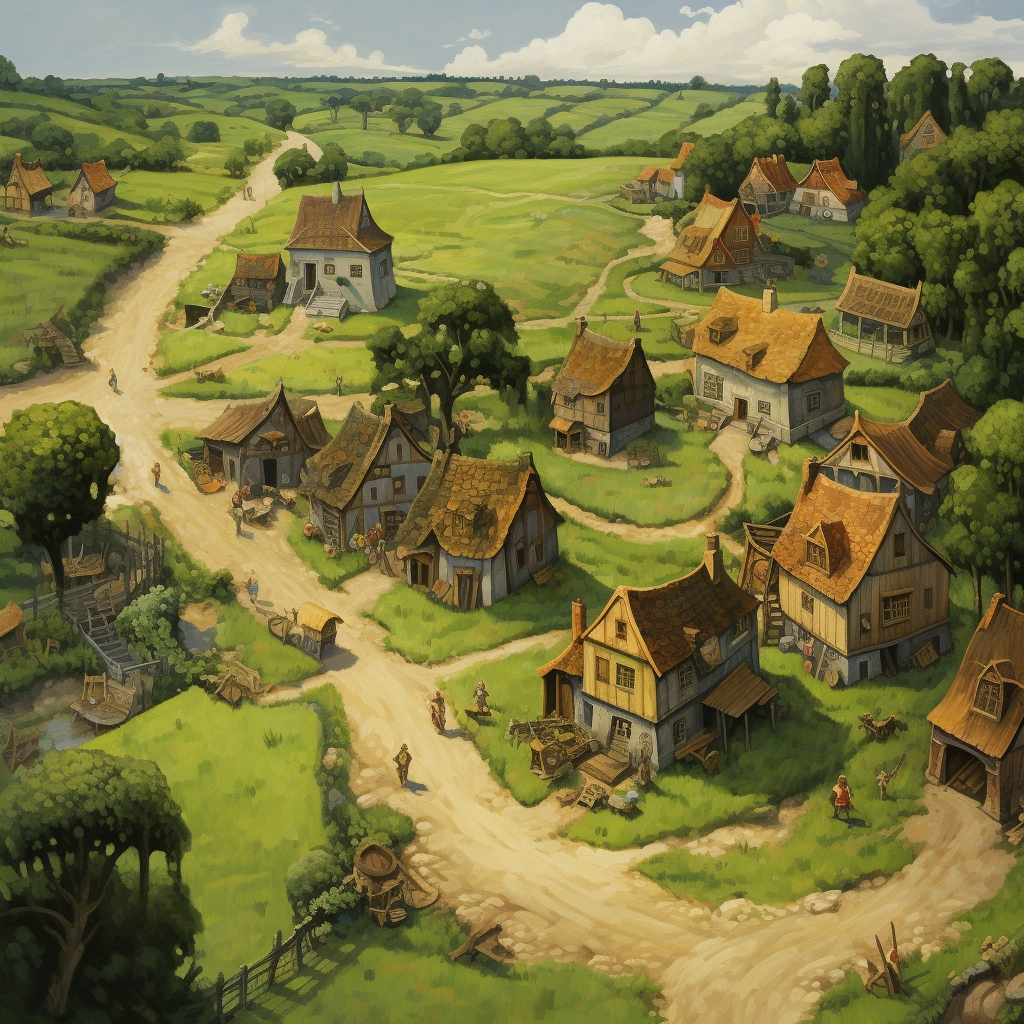
\includegraphics[scale=0.2]{BilderFuerBA/a_scatch_from_a_village_top_down.png}
   		 \caption{a scatch from a village, top down}
   		 \label{fig:Midjourney-Conceptart-Dorf}
\end{figure}
Nach der Erstellung der Hauptspielfigur, ist der nächste Schritt die Erstellung einer Spielwelt.
\\
Die Idee ist, ein Dorf in der Unreal Engine 5 zu erschaffen. In diesem Dorf befinden sich verschiedene Gebäude.
\\
In diesem Kapitel möchte ich zeigen, wie ich die Gebäude mit Hilfe verschiedener KI-Systeme in der Unreal Engine 5 realisiert habe. Ich werde in diesem Kapitel und in den folgenden Meilensteine nicht mehr detailliert auf alles wie bei der Erstellung der Hauptfigur eingehen, sondern nur auf Schritte, die sich im Prozess stark unterscheiden.
\\
Fachwerkhäuser repräsentieren etwas Mittelalterliches, und da die Renaissance zeitlich nach dem Mittelalter gegliedert ist, waren in Zeiten der Renaissance Fachwerkhäuser sehr weit verbreitet.
\\
Deshalb möchte ich diverse Fachwerkhäuser erschaffen und auf einer Landschaft verteilen, um eine Dorflandschaft zu erzeugen.
\\
\subsection{Erste Ansatz Fachwerkhäuser}%todo promts für die textur raussuchen
Mein erster Ansatz ist es, Häuser mit Hilfe von einem einfachen 3D-Modell umzusetzen, was ich in Blender erstellt habe. Dieses 3D-Modell bestand aus einem Quader mit einer Spitze. Kurz, ein einfaches Haus.
\\
Mit Midjourney habe ich Texturen erstellt, die Fachwerkhäuser nachempfunden sind. Diese Texturen und das einfache Haus wurden mit Hilfe von Blender verbunden.
\\
Folgend wurden die einfachen Fachwerkhäuser in Unreal Engine 5 Importiert und verteilt.
\\
Die erste Ansatz lässt funktioniert und man kann die Häuser frei auf einer Landschaft verteilen.
\\
\subsection{Moddelieren und texturieren Einfaches Haus mit Blender}
Ich habe mit Blender eine einfache Würfel mit Spitze modelliert was mein einfaches Fachwerkhaus darstellen soll. Dieses Einfache Fachwerkhaus habe ich eine Textur übergeben die ich mit Midjourney erzeugt habe.
\\
Beim Exportieren benötich ich keine Amature wie bei meiner Hauptfigur.
\\
Nach dem Exportieren kann ich die FBX datei in Unreal Engine 5 importieren.

\subsection{Zweiter Ansatz Fachwerkhäuser}%todo quellenn für valheim raussuchen
Eine Inspiration für meinen zweiten Ansatz ist Valheim, ein Survival-Spiel von den Coffee Stain Studios. In diesem Spiel gibt es ein Baukastensystem, in dem der Spieler sein eigenes Haus bauen kann.
\\
In Valheim kann der Spieler verschiedene Wände, Balken, Fußböden, Dächer und Materialarten auswählen, um damit seine Behausung zu gestalten.
\\
Hinzu kommen andere Elemente wie Zäune und Gemüse um ein Garten zu erschaffen, Werkbänke, Tische und Stühle um eine Inneneinrichtung zu kreieren und sogar Teppiche aus Tierfelle und Trophäen die man an die Wand hängen kann um eine Dekorative Charakter in die Behausung eines Spielers zu schaffen.
\\
Aus dieser Inspiration habe ich einen zweiten Ansatz entwickelt und zwar einen so genannten Dorfbaukasten.
\\
Dieser Dorfbaukasten besteht ebenfalls aus Wänden, Balken, Dächer, Dachgiebel, Fußböden und Tapeten.
\\
Aus meiner Beobachtung als Ein-Mann-Videospielentwickler, besteht ein Fachwerkhaus auch aus simplen Geometrien, wie zum Beispiel aus verschiedene Quader für Wände, Balken, Dach, Türen und Fenster. Der Dachgiebel von einem Fachwerkhaus ist ein dreieckiges Prisma. Diese einzelnen Elemente möchte ich nachbauen, so dass man in der Unreal Engine 5 einen Baukasten aus verschiedenen Einzelelementen verfügt um damit seine Fachwerkhäuser zu bauen. 
\\
Ein weiteres Ziel ist, diese einzelnen Elemente zu programmieren, damit die Materialeigenschaft sich untereinander unterscheiden. Das hat den Zweck, das die Spielwelt nicht zu monoton wirkt.
\\
Ein beispiel ist der Balken.
\\
Den Balken habe ich erstellt in dem ich ein neuen Blueprint Class vom typ Actor erstellt habe. Wenn man die Blueprint Class mit doppelklick öffnet, kann ich über das ADD unter Componets ein Cube hinzufügen.
\\
Diesen Cube habe ich in der X- und Y-Achse auf 0,4 Skaliert und somit habe ich meine Grundform für meinen Balken.
\\
Im Construction Script kann ich mit Hilfe von Nodes meinen Balken besondere Eigenschaften geben wie, zufällige Auswahl von Materialien oder das bestimmen der Länge mit Hilfe eines Parameters.
\\
\begin{figure}[h]
	%\centering
	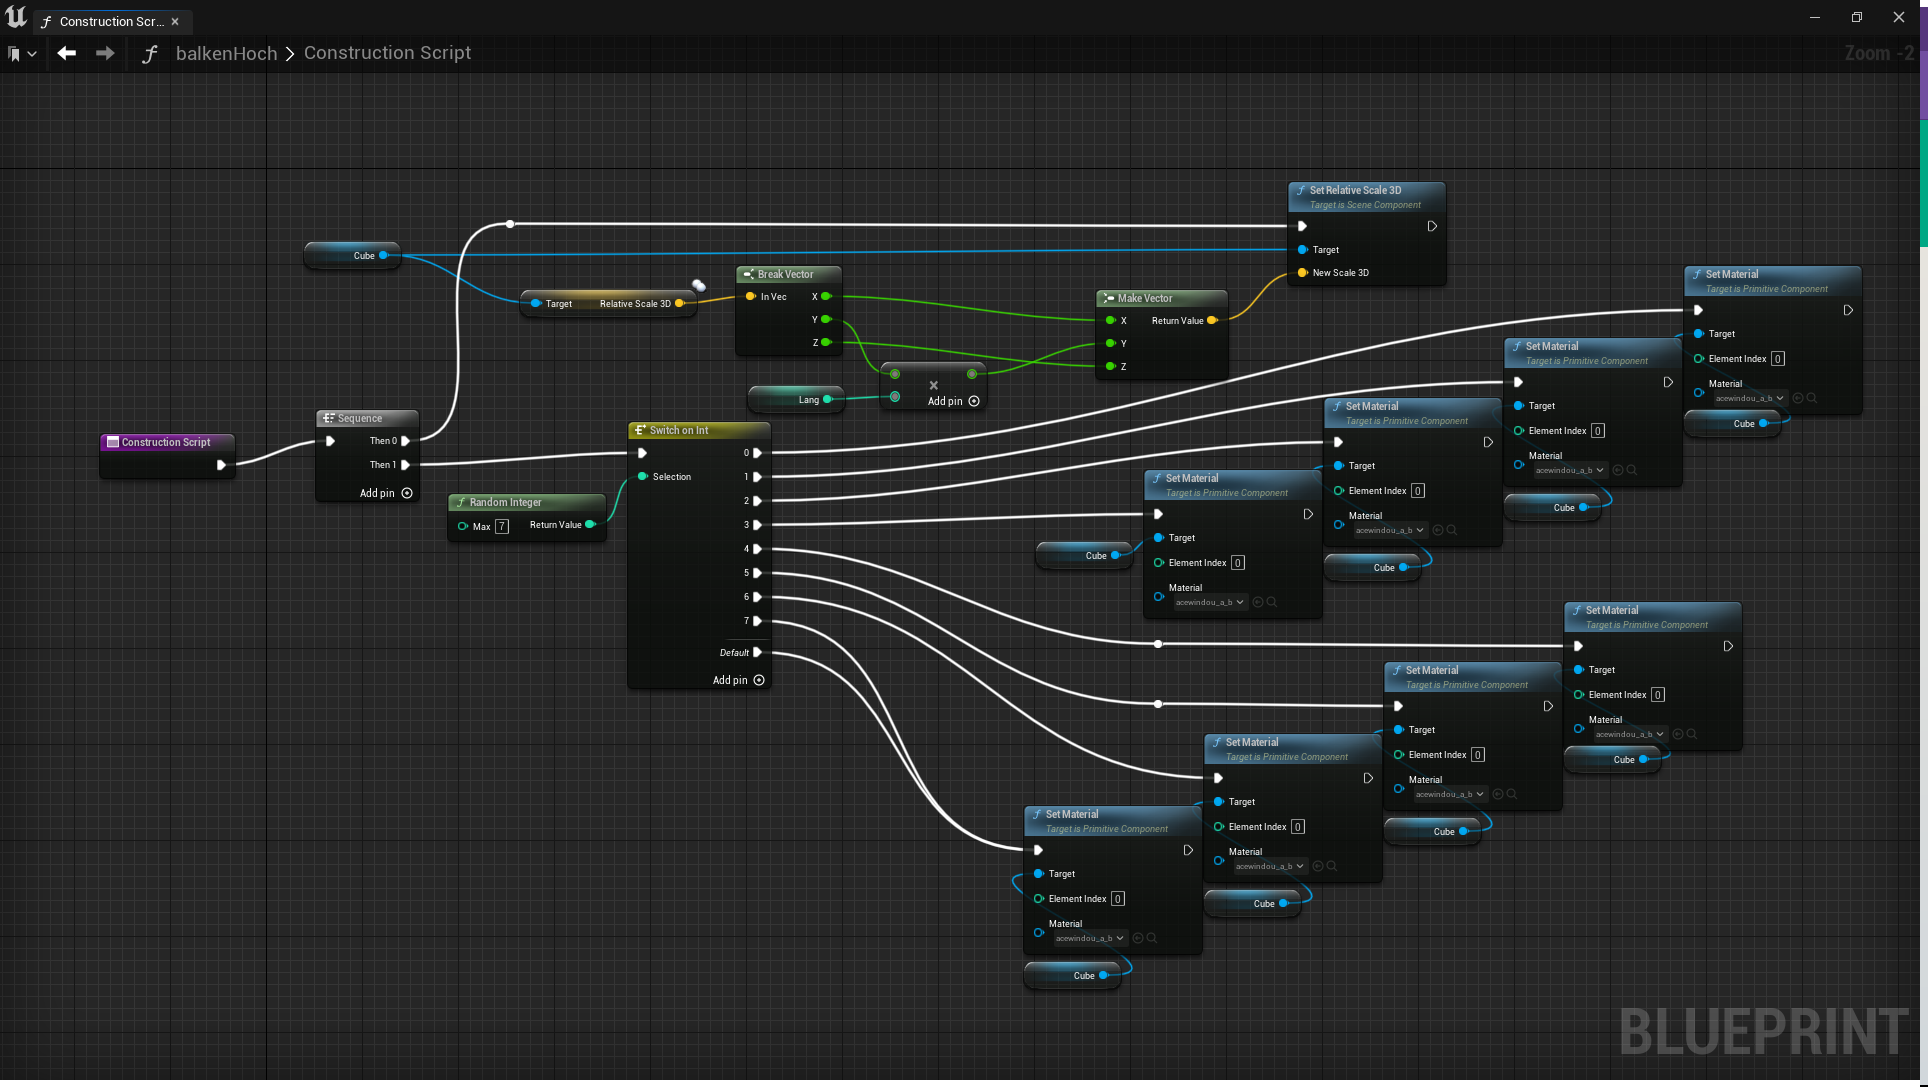
\includegraphics[width=14cm]{BilderFuerBA/Screenshot/UE5/balkenHochBP.png}
	\caption{UE5 Blueprint: Balken Hoch Construction Script}
	\label{UE5balkenHochBP}
\end{figure}

\section {Meilenstein: Nebenfiguren}
Beim dritten Meilenstein Nebenfiguren möchte ich gerne beschreiben, wie ich meine Nebenfiguren, kurz NPCs, erstellt habe. Ähnlich wie beim Erstellen der Hauptfigur habe ich durch Chat GPT mir verschiedene NPCs beschrieben lassen. Zu dieser Beschreibung gehörte Alter, Geschlecht, Beruf unnd charakterliche Eigenschaften.
\\
Mit diesen Beschreibungen habe ich mir einen Prompt mit hilfe der Midjourney-Formel überlegt und Midjourney hat mir Conceptgraphiken erzeugt. Nach mehreren Versuchen habe ich zwei Conzeptgraphiken bekommen die ich für PIFuHD verwenden kann.
\\
Nach dem ich PIFuHD die beiden Conzeptgraphiken übergeben habe, wu rden sie Wie bei der Hauptfigur in Blender der Polycount reduziert und Texturiert.  Stark verformete stellen die an den Händen und Füßen auftreten wurden im Eddit Mode, oder im Sculp Mode nachgebessert.
\\
Für den Prototyp impotiere ich die NPCs ohne Sceleton Mesh ein, da sie keine Laufanimation benötigen, sonder nur in der Spielwelt plaziert werden um mit dem Hauptcharakter zu reden.
\\
Dadurch das die NPC keine Sceleton Mesh besitzen ist auch gut zu erkennen, das die NPCs keine großen verformungen aufweisen wie die Hauptfigur. Die Verformung tritt z. B. in bereich der Hüfte sehr stark auf aufgrund der unterschiedlich gewichtete zuweisung der Vertices zu den einzelen Bones des Sceleton Mesh.


%\\\\\\\\\\\\\\\\\\\\\\\\\\\\\\\\\\\\\\\\\\\\\\\\\\\\ Dialogsystem\\\\\\\\\\\\\\\\\\\\\\\
%\\\\\\\\\\\\\\\\\\\\\\\\\\\\\\\\\\\\\\\\\\\\\\\\\\\\ Dialogsystem\\\\\\\\\\\\\\\\\\\\\\\
%\\\\\\\\\\\\\\\\\\\\\\\\\\\\\\\\\\\\\\\\\\\\\\\\\\\\ Dialogsystem\\\\\\\\\\\\\\\\\\\\\\\
\section {Meilenstein: Dialogsystem}
Um ein Dialogsystem in der Unreal Enginge 5 zu entwickeln habe ich mehrere Ansätze gebraucht.
 
Ansatz 1 mit ChatGPT
Ich habe ChatGPT dazu Aufgefordert mir ein Dialogsystem zu entwickeln damit mein Hauptcharakter mit den NPCs aus meinem Prototyp sich unterhalten können.
 
Ich habe versucht die Schritte umzusätzen die ChatGPT mir vorgegeben hat – Erfolglos.
 
Ansatz 2 Rechersche mit Suchmaschienen im Internet
Mit der Suchmaschiene Google
Durch Google bin ich auf ein Video auf Youtube gestoßen, was mir erklärt hat wie ich ein Dialogsystem in Unreal Engine 5 erstellt wird.
\\
Zu dem beschreibenen Dialogsystem wurde von mir noch ein Dilay in der Länge von dem Soundfile hinzugefügt und ein Bool, der auf false steht, falls eine Interaktion gerade nicht möglich ist, zu beispiel ein Charakter redet gerade noch. Dieser Bool soll verhindern, damit keine Dialoge schnell hintereinander gestartet werden und die Charaktere aussprechen lässt.
\\
Um die Sprachausgabe zu managen, braucht es ein Dialogsystem. Für das Dialogsystem habe ich
versucht, eine art Dialog System zu erschaffen, das man zum Beispiel aus der Sincefiction Spielereihe Mass Effect kennt. In dem der Spieler verschiedene Antworten- oder Fragemöglichkeiten besitzt. Das hat leider nicht von seiten ChatGPT nicht geklappt.
\\
Ich habe auch ChatGPT gefragt, wie ich ein Dialogsystem in der Unreal Engine 5 umsetzen kann. Auch das hat leider nicht funktioniert.
\\
An dieser Stelle ist gut zu erkennen das KI-Tool sehr gute ergebnisse erzeugen kann um ein Videospielprototypen zu entwickeln, aber KI-Systeme haben ihre Grenzen, sowie ich Als Ein-Mann-Videospiele-Entwickler auch grenzen habe in der Kompetenz diese Systeme zu bedienen.
\\
Das Problem, dass ich nicht weiß wie ein Dialogsystem entwickelt wurde, und ChatGPT mir ein Falsche lösung mir überreicht hat, habe ich durch die Suchmaschiene von Google und Youtube ein Tutorial gefunden wie ich ein Dialogsystem zwischen meiner Hauptfigur und den NPCs entwickeln kann.
\\
Also habe ich gegoogelt und auf youtube ein Tutorial gefunden.  	 Mit der andere Engine 5. Musste ich eine Schnittstelle, was zwischen den verschiedenen.  Actors wie zum Beispiel der Hauptfigur und den MPC.  Eine Schnittstelle bildet.    		 Diese Schnittstelle habe ich mit Blueprince umgesetzt. Ich musste auch bei blueprint m bei meiner Hauptfigur Martin Luther.  	 Etwas entwickeln und zwar habe ich ein Array erzeugt oder mehrere Arrays erzeugt. Die speichert, was gesagt wird, in Schriftform und was gesagt wird in.   Ausgabe.  In Sprachausgabe, in Soundausgabe.
\\
Ich habe eine Aktionsbutton hinzugefügt, was für was in diesem Beispiel der Buchstabe auf der Tastatur e ist.  Der sagt, Hey, ich möchte mit dir arbeiten.		 Ich habe einen Pool A erzeugt, die. Signalisiert. Hey, ich kann jetzt interagieren mit der Person oder gerade nicht.   		 Da das Dialogsystem. Vor z GPT unvollständig war habe ich mir noch andere Dialog Dialoge hinzu ausgedacht, andere Dialoge ausgedacht.  Und somit war das Dialogsystem auch schon fertig.



%\\\\\\\\\\\\\\\\\\\\\\\\\\\\\\\\\\\\\\\\\\\\\\\\\\\\ Sprachausgabe\\\\\\\\\\\\\\\\\\\\\\\
%\\\\\\\\\\\\\\\\\\\\\\\\\\\\\\\\\\\\\\\\\\\\\\\\\\\\ Sprachausgabe\\\\\\\\\\\\\\\\\\\\\\\
%\\\\\\\\\\\\\\\\\\\\\\\\\\\\\\\\\\\\\\\\\\\\\\\\\\\\ Sprachausgabe\\\\\\\\\\\\\\\\\\\\\\\
\section {Meilenstein: Sprachausgabe}
Nachdem ich das Dialogsystem erstellt und implementiert habe, fehlt nur noch der Inhalt, was die Charaktere miteinander als sich erzählen. Und zwar habe ich hier zwei neue Ki-Systeme benutzt, die vorher noch nicht zum Einsatz gekommen diese sind Voice AI und Adobe Enhance Speache.
\\
Voice AI ist ein KI-System, die Stimmen verändern kann. Zum Beispiel kann man seine Stimme so manipulieren, das sie wie die von Kanye West oder dem amtierende US-Präsident Joe Biden klingt.
\\
Adobe Enhanced ist ein KI-System, das deine gesprochene Stimme so klingen lässt, dass sie in einem hochwertigen Tonstudio aufgenommen wird.
\\
Meine Sprachaufnahmen verwende ich das Mikrofon von dem Logitech G35 Headset was seit 2014 nahezu täglich benutz wird.
\\
Durch die Kombination von Adobe Enhance Speech und Voice AI habe ich qualitativ hochwertige Sprach Dateien erzeugen können, die sonst ein hochwertiges Tonequipment und gute Dämmung in meinem Büro erzeugt hätten.
\\
Um die Stimmen für die NPCs zu erzeugen, habe ich drei verschiedene Experimente durchgeführt.
\\
\subsection{Erst Adobe Enhance Speache dann Voice AI}
Als erstes wurde der Klang meiner stimme mit Audacity und meinem Logitech G35 Headset aufgenommen.
\subsection{Erst Voice Ai dann Adobe Enhance Speech}
\subsection{Erst Adobe Enhance Speech dann Voice AI dann wieder Adobe Enhance Speech}
 
Experiment eins, erst Voice I gegeben und dann Adobe Anshan Speech. 		 Oder? Erst Adobe, Assange Speech und dann Voice AI.  Ich habe noch eine dritte.
\\
Variante ausprobiert, und zwar eine Art Sandwich Methode, indem ich meine Sounddatei, die ich mit Audacity aufgenommen habe, erst Adobe 1. Hand speech. Dann Voice I und dann wieder Adobe A Speech gegeben habe, um so eine Art zweifache Reinigung. Der Sprache oder der Sprachausgabe zu erhalten.     Mein persönliches bestes Ergebnis, was auch Zeittechnisch am. Sparsamsten war.  Ist erst.  Athan Speech zu benutzen und dann Voice I. Die dritte Version ist auch ok, aber es kann sein, dass danach sich die Stimme noch etwas künstlicher, Blecherner anhört.   Generell ist die Sprachausgabe sehr.  Gut.
\\
Und professionell anwendbar für mein Prototyp ist das eine Qualität, die ich früher nicht erreicht hatte können außer mit großen Aufwand und Kosten verbunden wie ZB das Kaufen eines 200€, Mikrofons und sehr guter Dämmung in meinem Aufnahmeraum. Ich habe die Aufnahmen bei einem sonnigen Tag während. Traktoren im Hintergrund arbeiten. Ich habe in meinem Arbeitszimmer. Ein Fenster aufgehabt. Das offenbar zu einem Bauernhof in meiner Nachbarschaft. Man kann Traktoren hören, man kann meine Frau hören, im Hintergrund, die in der Wohnung mit den Kindern sich beschäftigen und anhand Speech hat das alles herausgefiltert. Und ein gewisses Grundrauschen befindet sich auch nicht mehr und der Sound-Datei.
\\
Die Meilensteine.  Die ich hier in meiner Bachelor thesis beschreibe.  Sind nicht chronologisch sortiert, sondern nur logisch.  Ich habe das Dialogsystem und die Sprachausgabe gleichzeitig entwickelt und.  Implementiert.  Die Sprachausgabe, die ich hiermit mit Voice I und Adobe anhand Speech. Geschaffen habe, habe ich nun in das.  Dialogsystem was sich in dem vorigen Kapitel beschrieben habe. Implementiert. Ich habe die Sprachausgabe in das Array getan.		 In der andere Engine 5.
 
\section{Erstellung von Musik und Klängen}
\section{Erstellung von Animationen}
\section{Entwicklung der Spiellogik}